\documentclass[a4paper, 12pt]{article}
\usepackage{ae,aecompl}
\usepackage[T1]{fontenc}
\usepackage[utf8]{inputenc}
\usepackage{textcomp}
\usepackage{pgfplots}
\usepackage{anysize}
\marginsize{3.2cm}{2.8cm}{3cm}{2cm}
\usepackage{setspace}
\setstretch{1.2}
\frenchspacing
\pgfplotsset{compat=newest}
\pagestyle{empty}
\usepgfplotslibrary{ternary}
\usepackage{lscape}
\hyphenation{hő-mér-sék-let-füg-gé-sét}


\begin{document}

\section{Terner rendszer vizsgálata}
A háromkomponensű vagy terner rendszerek nem csak elméleti szempontból vetnek fel érdekes kérdéseket, de nagy gyakorlati jelentõségük is van, például a kohászatban, műanyagiparban.
Gondoljunk az olvadékokra, ötvözetekre, melyekben egy vagy több szilárd fázis tarthat egyensúlyt egy vagy két közös anyagot tartalmazó folyadékfázissal, vagy a polimerek oldására stb.
A terner rendszerekben a komponensek egymásban való kölcsönös oldhatósága különböző.
Minden ilyen rendszernél található olyan nyomás és/vagy hőmérséklet tartomány, melynél legalább két összetevő csak korlátosan elegyedik.
A harmadik komponens jelenléte - amennyiben ez részben vagy teljesen elegyedik a két másik komponenssel - megváltoztatja a két részben elegyedõ komponens kölcsönös oldhatóságát.

A terner rendszerek állapotának leírásához a nyomáson és hőmérsékleten kívül az összetételre van szükség, amennyiben a rendszerben kémiai reakció nem játszódik le.
Minthogy két komponens móltörtjének ismeretében a harmadik komponens móltörtje kiszámítható, ezért a szabadsági fokok száma egy ilyen rendszerben 4.
Adott hőmérsékleten és nyomáson tehát a rendszer állapotát a 2 összetétel adat egyértelműen meghatározza.
Ahhoz, hogy egy terner rendszer fázisdiagramját síkban ábrázolhassuk, két paramétert - célszerûen a nyomást és hőmérsékletet - állandónak kell vennünk.
Ez esetben a három komponens által meghatározott összetételt egyenlő oldalú háromszögben tüntethetjük fel.
A háromszög csúcsai jelentik a tiszta komponensekből álló egykomponensű rendszereket.
A könnyebb átláthatóságért célszerű a háromszögre egy körüljárási irányt meghatározni, amely a mi esetünkben az óramutató járásával ellentétes lesz. A háromszög oldalain az egyes komponensek móltörtjét - vagy tömegszázalékátszokás feltüntetni (\ref{fig:ccw}. ábra).

\begin{figure}
\centering
\begin{tikzpicture}
\begin{ternaryaxis}[
	xlabel=ecetsav m\%,
	ylabel=víz m\%,
	zlabel=kloroform m\%,
	minor tick num=9,
	grid=both,
	axis on top,
	xmin=0,
	xmax=100,
	ymin=0,
	ymax=100,
	zmin=0,
	zmax=100,
]
% plotdata/ternary_data.txt is a table of the form
%A_propene A_water A_IPA  B_propene B_water B_IPA
% 0.0009   0.9990  0      0.9333    0.0667  0
% 0.0009   0.9988  0.0002 0.9303    0.0665  0.0032
% 0.0011   0.9975  0.0013 0.9135    0.0673  0.0191
% 0.0013   0.9962  0.0024 0.8956    0.0693  0.0351
%...
	\addplot3[
		point meta=rand,
		tieline={
			each nth tie=8,
			tieline style={contour prepared}
		},
		fill=blue!10,
	]
	table [x=A_IPA,y=A_water,z=A_propene] 
		{plotdata/ternary_data.txt};
	\draw [decorate, decoration={brace,amplitude=15pt,raise=1pt}] (0,100) -- (50,0)  node [midway, xshift=-1mm, auto, swap, outer sep=10pt,font=\tiny]{debtee};
	\draw (0,100) -- (10,50)  node [midway, xshift=-1mm, auto, swap, outer sep=10pt,font=\tiny]{debtee};

\end{ternaryaxis}
\end{tikzpicture}
\caption{Terner rendszer diagramja.}
\label{fig:ccw}
\end{figure}

\begin{landscape}
\begin{figure}
\centering
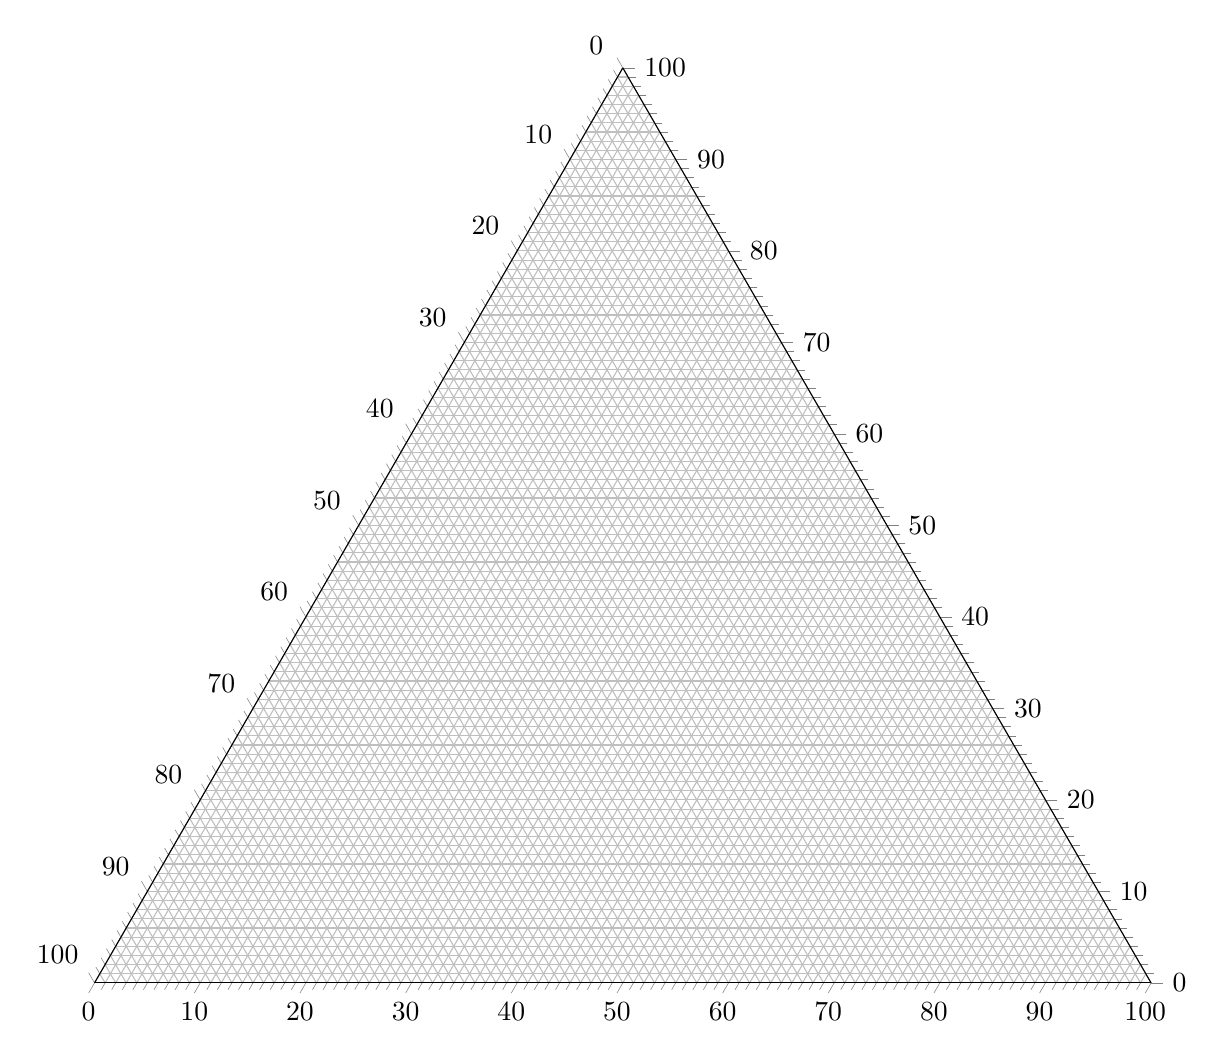
\begin{tikzpicture}
\begin{ternaryaxis}[minor tick num=9,grid=both,axis on top,xmin=0,xmax=100,ymin=0,ymax=100,zmin=0,zmax=100,width=15cm,height=15cm,]
% plotdata/ternary_data.txt is a table of the form
%A_propene A_water A_IPA  B_propene B_water B_IPA
% 0.0009   0.9990  0      0.9333    0.0667  0
% 0.0009   0.9988  0.0002 0.9303    0.0665  0.0032
% 0.0011   0.9975  0.0013 0.9135    0.0673  0.0191
% 0.0013   0.9962  0.0024 0.8956    0.0693  0.0351
%...
\end{ternaryaxis}
\end{tikzpicture}
%\caption{Terner diagram..}
\label{fig:ccw}
\end{figure}
\end{landscape}

\newpage
\pagebreak[4]
\section{Gyógyszerbomlás sebességének hőmérsékletfüggése}

\subsection{Bevezetés}
A gyakorlat során az Aspirin hidrolízisének kinetikailag elsőrendű reakciójának hőmérsékletfüggését vizsgáljuk.
A sebességi állandója a következőképpen adható meg:

\begin{equation}
\label{eq:divider}
        k
        =
        \frac
                {1}
                {t}
	\ln(\frac{z}{z-x})
\end{equation}

ahol $t$ az idő, $z$ a reagens (jelen esetben a Aspirin) kezdeti koncentrációja, $x$ pedig az elbomlott reagens koncentrációja.

A reakció sebessége vagy a sebességi állandó értéke függ a hõmérséklettől.
A hőmérsékletfüggést az Arrhenius egyenlet írja le:

\begin{equation}
\label{eq:divider}
        \frac
                {d\ln k}
                {dT}
	=
	\frac
		{E}
		{RT^2}
\end{equation}

melynek integrált alakja:

\begin{equation}
\label{eq:divider}
        k
        =
	A
	e^{-E/(RT)}
\end{equation}

illetve

\begin{equation}
\label{eq:divider}
        \lg k
        =
        \lg A
	-\frac{E}{2.303 RT}
\end{equation}

Az egyenletben $A$ a preexponenciális tényező, $E$ az aktiválási energia, és $R$ a gázállandó ($R = 8.314$ J/Kmol).
Az aktiválási energia meghatározható grafikus úton, ha az $\lg k - 1/T$ függvény meredekségét megmérjük és azt szorozzuk 2.303 $\times$ 8.314-el, amikor az $E$-t J/molban kapjuk meg.
Ha két hőmérsékleten megmérjük a reakciósebességi állandót ($k_1$-t és $k_2$-t $T_1$ és $T_2$ hőmérsékleten) az aktiválási energia a következő képlettel számítható ki:

\begin{equation}
	E
	=
	2.303
	\times
	8.314
	\lg
	\frac{k_1}{k_2}
	\frac{T_1 T_2}{T_1-T_2}
\end{equation}

\subsection{A gyakorlat kivitelezése}
Az Aspirin (acetilszalicilsav) hidrolízise kinetikailag elsőrendű folyamat és az alábbiak szerint játszódik le:
ábra: acetilszalicilsav és szalicilsav
A reakció szobahõmérsékleten igen lassú, ezért a méréseket magasabb hõmérsékleten végezzük.
A reakció sebességi állandójának meghatározásához ismerni kell a reaktáns vagy a termék koncentrációjának változását a reakcióidõvel.
Jelen reakcióban a képzõdõ szalicilsav Fe3+ ionokkal alkotott stabil ibolyaszínû komplexét határozzuk meg spektrofotometriás módszerrel.
A lúgos közegben lejátszódó reakcióelegybõl meghatározott reakcióidõnél ismert mennyiségû mintákat veszünk, a reakciót befagyasztjuk a hõmérséklet és a [OH-] hirtelen lecsökkentésével.
Az elõírt hígításokat követõen a szalicilsav Fe(III)-komplexének koncentrációját spektrofotometriás úton meghatározzuk.
A t = végtelen reakcióidõhöz tartozó termékkoncentrációkat, amelyek megfelelnek az Aspirin kezdeti koncentrációjának, igen nagy reakcióidõnél vett mintából lehet meghatározni.
A méréseket két hõmérsékleten kell végrehajtani, ezeket a gyakorlatvezetõ határozza meg a gyakorlat kezdetén.
(A reakció Arrhenius paramétereinek meghatározása érdekében ajánlott hõmérséklet 313 és 353 K (40 és 80 °C).)

2 db Aspirint külön-külön dörzsmozsárban elporítunk, és külön-külön fõzõpohárban kevés desztillált vízben oldunk, majd 25 cm3-es mérõlombikokba szûrjük és jelig töltjük (I. és II. törzsoldat).
A törzsoldatokon kívül még az alábbi oldatokat kell elkészíteni: 50-50 cm3 térfogatú 0.25 M HCl, 0.25 M NaOH, és 0.1 M HCl-ben oldott 0.1 M FeCl3.


Reakció alacsonyabb hõmérsékleten, pl. 313-323 K-en (a gyakorlatvezetõ határozza meg)

a) Az Aspirin kezdeti koncentrációjának (z) meghatározása:
Az I. sz. törzsoldatból 2 cm3 mintát csiszolatos dugós Erlenmeyer lombikba pipettázunk, hozzáadunk 3 cm3 0.25 M NaOH oldatot és a lombikot belehelyezzük a pontosan ismert hõmérsékletû termosztátba. 
A 60. percben a reakciót befagyasztjuk (a lombikot jeges vízbe és kevés desztillált vízzel mossuk, atot és desztillált vízzel 100 cm3-re hígítjuk.


b) A t idõpillanatig elbomlott Aspirin (x) koncentrációjának meghatározása:
Az I. törzsoldat maradékát a mérõlombikból csiszolatos dugós Erlenmeyer lombikba töltjük át (nem mossuk!), termosztátba helyezzük (t=0 perc), és a lombik kivétele nélkül a bomlás 15, 20, 25, 30 és 35. percében 2 cm3-es mintákat veszünk, amelyet az elõkészített 25 cm3-s mérõlombikokba töltünk.
A mintákhoz hozzáadunk 0.5 cm3 0.25 M HCl-at, 0.5 cm3 0.1 M FeCl3-at és 25 cm3 össztérfogatra hígítjuk õket desztillált vízzel.


Reakció magasabb hõmérsékleten, pl. 333-343 K-en (a gyakorlatvezetõ határozza meg)


a) Az Aspirin kezdeti koncentrációjának meghatározása:
A II. sz. törzsoldatból 2 cm3-t csiszolatos dugós Erlenmeyer lombikba pipettázunk, hozzáadunk 0.6 cm3 0.25 M NaOH-t és 15 cm3 desztillált vizet, majd a lombikot belehelyezzük az ismert hõmérsékletû termosztátba.
A 60. percben a reakciót befagyasztjuk, mintához lombik tartalmát 100 cm3-es mérõlombikba töltjük és kevés desztillált vízzel átmossuk, s a mintához hozzáadunk 1 cm3 0.25 M HCl-t, 2 cm3 0.1 M FeCl3-at, majd desztillált vízzel 25 cm3-re hígítjuk.

b) A t idõpontig elbomlott Aspirin koncentrációjának meghatározása:
A II. törzsoldat maradékát a mérõlombikból csiszolatos dugós Erlenmeyer lombikba töltjük át nem mossuk!), termosztátba helyezzük (t = 0 perc) és a lombik kivétele nélkül a bomlás 10, 15, 20, 25 és 30. percében 2 cm mintákat veszünk.
A 10, 15 és 20. percben vett mintákhoz hozzáadunk 0.5 cm3 0.25 M HCl-t és 0.5 cm3 0.l mólos FeCl3-at és 25 cm3-re hígítjuk desztillált vízzel.
Figyelem!
A kísérleteket célszerû úgy végezni, hogy a megadott térfogatú mérõlombikba elõre bepipettázzuk a megfelelõ mennyiségû sósavat és a FeCl3 oldatot, a lombikot 2/3-ad részéig feltöltjük desztillált vízzel, s jeges vízbe állítjuk. 
Az összes minta fogadására szükséges mérõlombikot készítsük így elõ és tegyük õket jeges vízbe.


Fényabszorpció mérése


Mind a kezdeti, mind a t idõpillanatban lévõ koncentráció meghatározása spektrofotometriásan történik.
A spektrofotométer kezelési leírása a készülék mellett megtalálható.


3. Beadandó eredmények

1. táblázat: A mérési és számított adatok táblázatosan
2. táblázat: A sebességi állandó hõmérsékletfüggése
3. A sebességi állandó hõmérsékletfüggésébõl határozzuk meg a sebességi állandó értékét 20 °C-on (293 K) grafikusan, ábrázolva a lg k - az l/T függvényében.
4. Az Arrhenius egyenlet integrált alakjába történõ behlyettesítéssel számtsuk ki az E aktiválási energiát és a preexponciális tényezõt:
E [kJ mol-1]
lgA[s-1]
A[s-1]

*standard deviációs számítása
s=….

\end{document}
